\documentclass[11pt]{article}
\usepackage[T1]{fontenc}
\usepackage{lmodern}
\usepackage[a4paper,left=25mm,right=30mm,top=22mm,bottom=24mm,marginparwidth=18mm]{geometry}
\usepackage{amsmath,amssymb,mathtools,stmaryrd}
\usepackage{tikz}
\usetikzlibrary{arrows.meta,calc,positioning}
\usepackage{caption}
\usepackage{xcolor}
\usepackage{marginnote}
\usepackage{microtype}
\usepackage{needspace}
\usepackage[hidelinks]{hyperref}
\definecolor{LeanTeal}{HTML}{087F72}
\definecolor{SourceGray}{HTML}{66736F}
\setlength{\parindent}{0pt}
\setlength{\parskip}{0.55em}
\setlength{\emergencystretch}{2em}
\newcommand{\leanmarker}[2]{%
  \Needspace{3\baselineskip}%
  \marginnote{\hyperlink{#1}{\color{LeanTeal}\fbox{\scriptsize Lean}}}%
  \hypertarget{#1}{\textbf{#2.}}%
}
\newcommand{\sourcepage}[1]{\par\medskip\noindent\textcolor{SourceGray}{\scriptsize Source PDF page #1}\par\smallskip}
\pagestyle{plain}
\begin{document}
\begin{center}\LARGE\bfseries Domains collectively\par\medskip
\large Lean 4 Formalization Companion -- Chapter 3\end{center}
\medskip
\noindent\textit{This project-generated reading copy contains reviewed mathematical items, short source locators, and redrawn diagrams. It does not reproduce the original PDF or automatic OCR prose. Click a Lean tag in the web reader to open the mapped Lean declaration.}
\bigskip\hrule\bigskip
\section*{Section 3.1}
\sourcepage{34}
\leanmarker{def-3-1-1}{Definition 3.1.1} Let $P$ and $Q$ be posets. A pair $s:P\to Q$, $r:Q\to P$ of monotone functions is called a \emph{monotone section retraction pair} if $r\circ s$ is the identity on $P$. In this situation we will call $P$ a monotone retract of $Q$.

If $P$ and $Q$ are dcpo's and if both functions are continuous then we speak of a \emph{continuous section retraction pair}.

We will omit the qualifying adjective ``monotone'', respectively ``continuous'', if the properties of the functions are clear from the context. We will also use \emph{s-r-pair} as a shorthand.

One sees immediately that in an s-r-pair the retraction is surjective and the section is injective, so our intuition about $P$ being both a sub-object and a quotient of $Q$ is justified. In such a situation $P$ inherits many properties from $Q$:

\leanmarker{prop-3-1-2}{Proposition 3.1.2} Let $P$ and $Q$ be posets and let $s:P\to Q$, $r:Q\to P$ be a monotone section retraction pair.
\begin{enumerate}
\item Let $A$ be any subset of $P$. If $s(A)$ has a supremum in $Q$ then $A$ has a supremum in $P$. It is given by
\[
  r\left(\bigvee s(A)\right).
\]
Similarly for the infimum.
\item If $Q$ is a (pointed) dcpo, a semilattice, a lattice or a complete lattice then so is $P$.
\end{enumerate}

\emph{Proof.} Because of $r\circ s=\operatorname{id}_P$ and the monotonicity of $r$ it is clear that $r(\bigvee s(A))$ is an upper bound for $A$. Let $x$ be another such. Then by the monotonicity of $s$ we have that $s(x)$ is an upper bound of $s(A)$ and hence it is above $\bigvee s(A)$. So we get
\[
  x = r(s(x)) \sqsupseteq r\left(\bigvee s(A)\right).
\]
The property of being a (pointed) dcpo, semilattice, etc., is defined through the existence of suprema or infima of certain subsets. The shape of these subsets is preserved by monotone functions and so (2) follows from (1).

Let us now turn to continuous section retraction pairs.

\leanmarker{lemma-3-1-3}{Lemma 3.1.3} Let $(s,r)$ be a continuous section retraction pair between dcpo's $D$ and $E$ and let $B$ be a basis for $E$. Then $r(B)$ is a basis for $D$.

\emph{Proof.} Let $c\in B$ be an approximant to $s(x)$ for $x\in D$. We show that $r(c)$ approximates $x$. To this end let $A$ be a directed subset of $D$ with $\bigvee^{\uparrow} A\sqsupseteq x$. By the continuity of $s$ we have
\[
  \bigvee^{\uparrow} s(A)=s\left(\bigvee^{\uparrow} A\right)\sqsupseteq s(x)
\]
and so for some $a\in A$, $s(a)\sqsupseteq c$ must hold. This implies $a=r(s(a))\sqsupseteq r(c)$. The continuity of $r$ gives us that $x$ is the supremum of $r(B_{s(x)})$.

\sourcepage{35}
\leanmarker{thm-3-1-4}{Theorem 3.1.4} A retract of a continuous domain via a continuous s-r-pair is continuous.

The analogous statement for algebraic domains does not hold in general. Instead of constructing a particular counterexample, we use our knowledge about the ideal completion to get a general, positive result which implies this negative one.

\leanmarker{thm-3-1-5}{Theorem 3.1.5} Every $(\omega\text{-})$continuous domain is the retract of an $(\omega\text{-})$algebraic domain via a continuous s-r-pair.

In more detail, we have:

\leanmarker{prop-3-1-6}{Proposition 3.1.6} Let $D$ be a continuous domain with basis $B$. Then the maps
\[
  s:D\to \operatorname{Idl}(B,\sqsubseteq),\quad x\mapsto B_x
\]
and
\[
  r:\operatorname{Idl}(B,\sqsubseteq)\to D,\quad A\mapsto \bigvee^{\uparrow} A
\]
constitute a continuous section retraction pair between $D$ and $\operatorname{Idl}(B,\sqsubseteq)$.

\emph{Proof.} The continuity of $r$ follows from general associativity, Proposition 2.1.4, and the fact that directed suprema in $\operatorname{Idl}(B)$ are directed unions. For the continuity of $s$ we use the interpolation property in the form of Proposition 2.2.16(2).

\leanmarker{prop-3-1-7}{Proposition 3.1.7}
\begin{enumerate}
\item The image of a continuous idempotent map $f$ on a dcpo $D$ is a dcpo. The suprema of directed subsets of $\operatorname{im}(f)$, calculated in $\operatorname{im}(f)$, coincide with those calculated in $D$. The inclusion $\operatorname{im}(f)\to D$ is Scott-continuous.
\item The set of all continuous idempotent functions on a dcpo is again a dcpo.
\end{enumerate}

\emph{Proof.} (1) The first part follows from Proposition 3.1.2 because the inclusion is surely monotone. For the second part let $A$ be a directed set contained in $\operatorname{im}(f)$. We need to see that $\bigvee^{\uparrow} A$ belongs to $\operatorname{im}(f)$ again. This holds because $f$ is continuous:
\[
  \bigvee^{\uparrow} A = \bigvee^{\uparrow} f(A) = f\left(\bigvee^{\uparrow} A\right).
\]
(2) Let $(f_i)_{i\in I}$ be a directed family of continuous idempotents. For any $x\in D$ we can calculate
\[
\begin{aligned}
\left(\bigvee^{\uparrow}_{i\in I} f_i\right)\circ
\left(\bigvee^{\uparrow}_{j\in I} f_j\right)(x)
&= \bigvee^{\uparrow}_{i\in I} f_i\left(\bigvee^{\uparrow}_{j\in I} f_j(x)\right) \\
&= \bigvee^{\uparrow}_{i\in I}\bigvee^{\uparrow}_{j\in I} f_i(f_j(x)) \\
&= \bigvee^{\uparrow}_{i\in I} f_i(f_i(x)) \\
&= \bigvee^{\uparrow}_{i\in I} f_i(x).
\end{aligned}
\]
Hence the supremum of continuous idempotents is again an idempotent function. We have proved in Proposition 2.1.18 that it is also continuous.

If $f$ is a continuous idempotent map on a continuous domain $D$ then we know that its image is again continuous. But it is not true that the order of approximation on $\operatorname{im}(f)$ is the restriction of the order of approximation on $D$. For example, every constant map is continuous and idempotent. Its image is an algebraic domain with one element, which is therefore compact. But surely not every element of a continuous domain is compact. However, we can say something nice about the Scott-topology on the image:

\sourcepage{36}
\leanmarker{prop-3-1-8}{Proposition 3.1.8} If $f$ is a continuous idempotent function on a dcpo $D$ then the Scott-topology on $\operatorname{im}(f)$ is the restriction of the Scott-topology on $D$ to $\operatorname{im}(f)$.

\emph{Proof.} This follows immediately because a continuous idempotent function $f$ gives rise to a continuous s-r-pair between $\operatorname{im}(f)$ and $D$.

Useful examples of idempotent self-maps are retractions $\operatorname{ret}_x$ onto principal ideals. They are given by
\[
  \operatorname{ret}_x(y)=
  \begin{cases}
    y, & \text{if } y\sqsubseteq x,\\
    x, & \text{otherwise.}
  \end{cases}
\]
Their continuity follows from the fact that $\downarrow x$ is always Scott-closed. Dually, we can define a retraction onto a principal filter $\uparrow c$. It is Scott-continuous if (but not only if) its generator $c$ is compact.

\begin{figure}[ht]
\centering
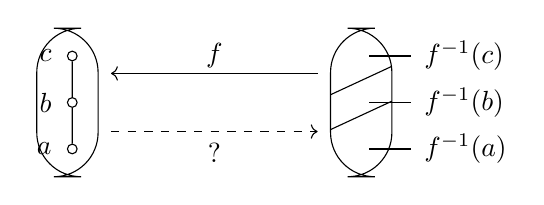
\begin{tikzpicture}[scale=0.82]
  \tikzset{dot/.style={circle,draw,fill=white,inner sep=0pt,minimum size=3.5pt}}
  \draw[rounded corners=16pt] (-2.8,-1.15) rectangle (-1.85,1.15);
  \node[dot] (c) at (-2.25,0.72) {};
  \node[dot] (b) at (-2.25,0) {};
  \node[dot] (a) at (-2.25,-0.72) {};
  \node[left] at (-2.42,0.72) {$c$};
  \node[left] at (-2.42,0) {$b$};
  \node[left] at (-2.42,-0.72) {$a$};
  \draw (a)--(b)--(c);

  \draw[rounded corners=16pt] (1.75,-1.15) rectangle (2.7,1.15);
  \draw (1.75,-0.42)--(2.7,0.02);
  \draw (1.75,0.12)--(2.7,0.56);
  \draw (2.35,0.72)--(3.0,0.72);
  \draw (2.35,0)--(3.0,0);
  \draw (2.35,-0.72)--(3.0,-0.72);
  \node[right] at (3.05,0.72) {$f^{-1}(c)$};
  \node[right] at (3.05,0) {$f^{-1}(b)$};
  \node[right] at (3.05,-0.72) {$f^{-1}(a)$};

  \draw[->] (1.55,0.45)--(-1.65,0.45);
  \node at (-0.05,0.72) {$f$};
  \draw[->,dashed] (-1.65,-0.45)--(1.55,-0.45);
  \node at (-0.05,-0.78) {?};
\end{tikzpicture}
\caption*{Figure 7: The right inverse problem for a surjective function.}
\end{figure}

\sourcepage{37}
\leanmarker{def-3-1-9}{Definition 3.1.9} (preliminary) Let $P$ and $Q$ be posets and let $l:P\to Q$ and $u:Q\to P$ be monotone functions. We say that $(l,u)$ is an \emph{adjunction} between $P$ and $Q$ if for every $x\in P$ we have that $l(x)$ is the least element of $u^{-1}(\uparrow x)$.

This definition is simple and easy to motivate. But it brings out just one aspect of adjoint pairs, namely, that $l$ is uniquely determined by $u$. There is much more:

\leanmarker{prop-3-1-10}{Proposition 3.1.10} Let $P$ and $Q$ be posets and $l:P\to Q$ and $u:Q\to P$ be monotone functions. Then the following are equivalent:
\begin{enumerate}
\item $\forall x\in P.\ l(x)=\min(u^{-1}(\uparrow x))$,
\item $\forall y\in Q.\ u(y)=\max(l^{-1}(\downarrow y))$,
\item $l\circ u\sqsubseteq \operatorname{id}_Q$ and $u\circ l\sqsupseteq \operatorname{id}_P$,
\item $\forall x\in P\ \forall y\in Q.\ (x\sqsubseteq u(y) \Longleftrightarrow l(x)\sqsubseteq y)$.
\end{enumerate}
For $(4)\Rightarrow(1)$ the monotonicity of $u$ and $l$ is not needed.

\emph{Proof.} $(1)\Rightarrow(2)$ Pick an element $y\in Q$. Then because $u(y)\sqsubseteq u(y)$ we have from (1) that $l(u(y))\sqsubseteq y$ holds. So $u(y)$ belongs to $l^{-1}(\downarrow y)$. Now let $x'$ be any element of $l^{-1}(\downarrow y)$, or, equivalently, $l(x')\sqsubseteq y$. Using (1) again, we see that this can only happen if $u(y)\sqsupseteq x'$ holds. So $u(y)$ is indeed the largest element of $l^{-1}(\downarrow y)$. The converse is proved analogously, of course.

(1) and (2) together immediately give both (3) and (4). From (3) we get (4) by applying the monotone map $l$ to the inequality $x\sqsubseteq u(y)$ and using $l\circ u\sqsubseteq \operatorname{id}_Q$.

Assuming (4) we see immediately that $l(x)$ is a lower bound for $u^{-1}(\uparrow x)$. But because $l(x)\sqsubseteq l(x)$ and hence $x\sqsubseteq u(l(x))$ we have that $l(x)$ also belongs to $u^{-1}(\uparrow x)$. We get the monotonicity of $l$ as follows: if $x\sqsubseteq x'$ holds in $P$, then because $l(x')\sqsubseteq l(x')$ we have $x'\sqsubseteq u(l(x'))$ and by transitivity $x\sqsubseteq u(l(x'))$. Using (4) again, we get $l(x)\sqsubseteq l(x')$.

We conclude that despite the lopsided definition, the situation described by an adjunction is completely symmetric. And indeed, adjunctions are usually introduced using either (3) or (4).

\sourcepage{38}
\leanmarker{def-3-1-11}{Definition 3.1.11} (official) Let $P$ and $Q$ be posets and let $l:P\to Q$ and $u:Q\to P$ be functions. We say that $(l,u)$ is an \emph{adjunction} between $P$ and $Q$ if for all $x\in P$ and $y\in Q$ we have
\[
  x\sqsubseteq u(y) \Longleftrightarrow l(x)\sqsubseteq y.
\]
We call $l$ the lower and $u$ the upper adjoint and write $l:P\rightleftarrows Q:u$.

\leanmarker{prop-3-1-12}{Proposition 3.1.12} Let $l:P\rightleftarrows Q:u$ be an adjunction between posets.
\begin{enumerate}
\item $u\circ l\circ u=u$ and $l\circ u\circ l=l$,
\item the image of $u$ and the image of $l$ are order-isomorphic. The isomorphisms are given by the restrictions of $u$ and $l$ to $\operatorname{im}(l)$ and $\operatorname{im}(u)$, respectively,
\item $u$ is surjective $\Longleftrightarrow u\circ l=\operatorname{id}_P \Longleftrightarrow l$ is injective,
\item $l$ is surjective $\Longleftrightarrow l\circ u=\operatorname{id}_Q \Longleftrightarrow u$ is injective,
\item $l$ preserves existing suprema, $u$ preserves existing infima.
\end{enumerate}

\emph{Proof.} (1) We use Proposition 3.1.10(3) twice:
\[
  u=\operatorname{id}_P\circ u \sqsubseteq (u\circ l)\circ u
    =u\circ(l\circ u)\sqsubseteq u\circ\operatorname{id}_Q=u.
\]
(2) The equations from (1) say precisely that on the images of $u$ and $l$, $u\circ l$ and $l\circ u$, respectively, act like identity functions.

(3) If $u$ is surjective then we can cancel $u$ on the right in the equation $u\circ l\circ u=u$ and get $u\circ l=\operatorname{id}_P$. From this it follows that $l$ must be injective.

(5) Let $x=\bigvee A$ for $A\subseteq P$. By monotonicity, $l(x)\sqsupseteq l(a)$ for each $a\in A$. Conversely, let $y$ be any upper bound of $l(A)$. Then $u(y)$ is an upper bound for each $u(l(a))$ which in turn is above $a$. So $u(y)\sqsupseteq \bigvee A=x$ holds and this is equivalent to $y\sqsupseteq l(x)$.

The last property in the preceding proposition may be used to define an adjunction in yet another way, the only prerequisite being that there are enough sets with an infimum (or supremum). This is the Adjoint Functor Theorem for posets.

\leanmarker{prop-3-1-13}{Proposition 3.1.13} Let $f:L\to P$ be a monotone function from a complete lattice to a poset. Then the following are equivalent:
\begin{enumerate}
\item $f$ preserves all infima,
\item $f$ has a lower adjoint.
\end{enumerate}
And similarly: $f$ preserves all suprema if and only if $f$ has an upper adjoint.

\emph{Proof.} We already know how to define a candidate for a lower adjoint $g$; we try
\[
  g(x)=\bigwedge f^{-1}(\uparrow x).
\]
All that remains is to show that $g(x)$ belongs to $f^{-1}(\uparrow x)$. This follows because $f$ preserves meets:
\[
  f(g(x))=f\left(\bigwedge f^{-1}(\uparrow x)\right)
    =\bigwedge f(f^{-1}(\uparrow x))\sqsupseteq \bigwedge\uparrow x=x.
\]

This proposition gives us a way of recognizing an adjoint situation in cases where only one function is explicitly given. It is then useful to have a notation for the missing mapping. We write $f^*$ for the upper and $f_*$ for the lower adjoint of $f$.

Now it is high time to come back to domains and see what all this means in our setting.

\sourcepage{39}
\leanmarker{prop-3-1-14}{Proposition 3.1.14} Let $l:D\rightleftarrows E:u$ be an adjunction between dcpo's.
\begin{enumerate}
\item $l$ is Scott-continuous.
\item If $u$ is Scott-continuous then $l$ preserves the order of approximation.
\item If $D$ is continuous then the converse of (2) is also true.
\end{enumerate}

\emph{Proof.} Continuity of the lower adjoint follows from Proposition 3.1.12(5). So let $x\ll y$ be elements in $D$ and let $A$ be a directed subset of $E$ such that $l(y)\sqsubseteq \bigvee^{\uparrow} A$ holds. This implies $y\sqsubseteq u(\bigvee^{\uparrow}A)$ and from the continuity of $u$ we deduce $y\sqsubseteq \bigvee^{\uparrow}u(A)$. Hence some $u(a)$ is above $x$ which, going back to $E$, means $l(x)\sqsubseteq a$.

(3) For the converse let $A$ be any directed subset of $E$. Monotonicity of $u$ yields $\bigvee^{\uparrow}u(A)\sqsubseteq u(\bigvee^{\uparrow} A)$. In order to show that the other inequality also holds, we prove that $\bigvee^{\uparrow}u(A)$ is above every approximant to $u(\bigvee^{\uparrow}A)$. Indeed, if $x\ll u(\bigvee^{\uparrow}A)$ we have
\[
  l(x)\ll l\left(u\left(\bigvee^{\uparrow}A\right)\right)\sqsubseteq \bigvee^{\uparrow}A
\]
by assumption. So some $a$ is above $l(x)$ and for this $a$ we have $x\sqsubseteq u(a)\sqsubseteq \bigvee^{\uparrow}u(A)$.

\leanmarker{def-3-1-15}{Definition 3.1.15} Let $D$ and $E$ be dcpo's and let $e:D\to E$ and $p:E\to D$ be continuous functions. We say that $(e,p)$ is a \emph{continuous embedding projection pair} (or \emph{e-p-pair}) if
\[
  p\circ e=\operatorname{id}_D \quad\text{and}\quad e\circ p\sqsubseteq \operatorname{id}_E.
\]

We note that the section retraction pair between a continuous domain and its ideal completion as constructed in Section 3.1.1 is really an embedding projection pair.

From the general theory of adjunctions and retractions we already know quite a bit about e-p-pairs. The embedding is injective, $p$ is surjective, $e$ preserves existing suprema and the order of approximation, $p$ preserves existing infima, $D$ is continuous if $E$ is continuous, and, finally, embeddings and projections uniquely determine each other. Because of this last property the term ``embedding'' has a well-defined meaning; it is an injective function which has a Scott-continuous upper adjoint.

An injective lower adjoint also reflects the order of approximation:

\leanmarker{prop-3-1-16}{Proposition 3.1.16} Let $e:D\rightleftarrows E:p$ be an e-p-pair between dcpo's and let $x$ and $y$ be elements of $D$. Then $e(x)\ll e(y)$ holds in $E$ if and only if $x$ approximates $y$ in $D$.

\sourcepage{40}
\leanmarker{prop-3-1-17}{Proposition 3.1.17} Let $D$ be a dcpo.
\begin{enumerate}
\item $[D\xrightarrow{\downarrow}D]$ is a dcpo.
\item If $p$ is a kernel operator on $D$ then for all $x\in D$ we have
\[
  p(x)=\max\{y\in\operatorname{im}(p)\mid y\sqsubseteq x\}.
\]
\item The image of a kernel operator is closed under existing suprema.
\item $\ll_{\operatorname{im}(p)}=(\ll_D)\cap(\operatorname{im}(p)\times\operatorname{im}(p))$.
\item For kernel operators $p,p'$ on $D$ we have $p\sqsubseteq p'$ if and only if $\operatorname{im}(p)\subseteq\operatorname{im}(p')$.
\end{enumerate}

\emph{Proof.} (1) is proved as Proposition 3.1.7 and (2) follows because $p$ together with the inclusion of $\operatorname{im}(p)$ into $D$ form an adjunction. This also shows (4). Finally, (3) and (5) are direct consequences of (2).

\sourcepage{41}
\leanmarker{prop-3-1-18}{Proposition 3.1.18} Let $D$ be an algebraic domain and let $c:D\to D$ be a monotone idempotent function above $\operatorname{id}_D$. Then $\operatorname{im}(c)$ is again an algebraic domain if and only if it is closed under directed suprema.

The reader will no doubt recognize this statement as being a reformulation and generalization of our example of inductive closure systems from Chapter 2, Proposition 2.2.9. It is only consequent to call $D$ a quotient domain of the continuous domain $E$ if there exists an i-c-pair $e:D\leftrightarrows E:c$.

\clearpage
\section*{Section 3.2}
\sourcepage{42}
\leanmarker{def-3-2-1}{Definition 3.2.1} The cartesian product of two dcpo's $D$ and $E$ is given by the following data:
\[
  D\times E=\{\langle x,y\rangle\mid x\in D,\ y\in E\},
\]
\[
  \langle x,y\rangle\sqsubseteq\langle x',y'\rangle
  \quad\text{if and only if}\quad
  x\sqsubseteq x'\ \text{and}\ y\sqsubseteq y'.
\]
This is just the usual product of sets, augmented by the coordinatewise order. Through induction, we can define the cartesian product for finite non-empty collections of dcpo's. For the product over the empty index set we define the result to be a fixed one-element dcpo $I$.

\leanmarker{prop-3-2-2}{Proposition 3.2.2} The cartesian product of dcpo's is a dcpo. Suprema and infima are calculated coordinatewise.

With each product $D\times E$ there are associated two projections:
\[
  \pi_1:D\times E\to D \quad\text{and}\quad \pi_2:D\times E\to E.
\]
These projections are always surjective but they are upper adjoints only if $D$ and $E$ are pointed. So there is a slight mismatch with Section 3.1.4 here. Given a dcpo $F$ and continuous functions $f:F\to D$ and $g:F\to E$, we denote the mediating morphism from $F$ to $D\times E$ by $\langle f,g\rangle$. It maps $x\in F$ to $\langle f(x),g(x)\rangle$.

\leanmarker{prop-3-2-3}{Proposition 3.2.3} Projections and mediating morphisms are continuous.

If $f:D\to D'$ and $g:E\to E'$ are Scott-continuous, then so is the mediating map
\[
  \langle f\circ\pi_1,\ g\circ\pi_2\rangle:D\times E\to D'\times E'.
\]
The common notation for it is $f\times g$. Since our construction is completely explicit, we have thus defined a functor in two variables on $\mathbf{DCPO}$.

\leanmarker{prop-3-2-4}{Proposition 3.2.4} Let $D$ and $E$ be dcpo's.
\begin{enumerate}
\item A tuple $\langle x,y\rangle$ approximates a tuple $\langle x',y'\rangle$ in $D\times E$ if and only if $x$ approximates $x'$ in $D$ and $y$ approximates $y'$ in $E$.
\item If $B$ and $B'$ are bases for $D$ and $E$, respectively, then $B\times B'$ is a basis for $D\times E$.
\item $D\times E$ is continuous if and only if $D$ and $E$ are.
\item $K(D\times E)=K(D)\times K(E)$.
\end{enumerate}

The categorical aspect of the cartesian product is quite pleasing; it is a categorical product in each case. But we can say even more.

\leanmarker{lemma-3-2-5}{Lemma 3.2.5} Let $\mathcal{C}$ be a full subcategory of $\mathbf{DCPO}$ or $\mathbf{DCPO}_{\bot!}$ which has finite products. Then these are isomorphic to the cartesian product.

In a restricted setting this was first observed in [Smy83a]. The general proof may be found in [Jun89]. A useful property which does not follow from general categorical or topological considerations is the following.

\sourcepage{43}
\leanmarker{lemma-3-2-6}{Lemma 3.2.6} A function $f:D\times E\to F$ is continuous if and only if it is continuous in each variable separately.

\emph{Proof.} Assume $f:D\times E\to F$ is separately continuous. Then $f$ is monotone, because given $(x,y)\sqsubseteq(x',y')$ we can fill in $(x,y')$ and use coordinatewise monotonicity twice. The same works for continuity: if $A\subseteq D\times E$ is directed then
\[
\begin{aligned}
\bigvee_{(x,y)\in A}^{\uparrow} f(x,y)
&= \bigvee_{x\in\pi_1(A)}^{\uparrow}\ \bigvee_{y\in\pi_2(A)}^{\uparrow} f(x,y)\\
&= \bigvee_{x\in\pi_1(A)}^{\uparrow} f\left(x,\bigvee_{y\in\pi_2(A)}^{\uparrow}y\right)\\
&= f\left(\bigvee_{x\in\pi_1(A)}^{\uparrow}x,\bigvee_{y\in\pi_2(A)}^{\uparrow}y\right)\\
&= f\left(\bigvee^{\uparrow}A\right).
\end{aligned}
\]
This proves the interesting direction.

\begin{figure}[ht]
\centering
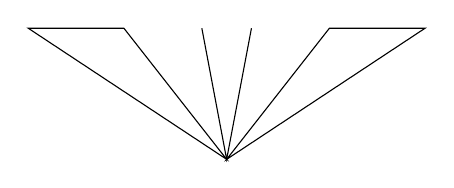
\begin{tikzpicture}[scale=0.9]
  \coordinate (bot) at (0,0);
  \draw (-2.8,1.85)--(-1.45,1.85)--(bot)--cycle;
  \draw (2.8,1.85)--(1.45,1.85)--(bot)--cycle;
  \draw (-0.35,1.85)--(bot)--(0.35,1.85);
\end{tikzpicture}
\caption*{Figure 8: The coalesced sum of two pointed dcpo's.}
\end{figure}

\sourcepage{44}
\leanmarker{lemma-3-2-7}{Lemma 3.2.7} Let $\mathcal{C}$ be a cartesian closed full subcategory of $\mathbf{DCPO}$. The exponential of two objects $D$ and $E$ of $\mathcal{C}$ is isomorphic to $[D\to E]$.

Let us now turn to the theme of approximation in function spaces. The reader should brace himself for a profound disappointment: even for algebraic domains it may be the case that the order of approximation on the function space is empty. Exercise 3.3.12(11) discusses an example. This fact together with Lemmas 3.2.5 and 3.2.7 implies that neither $\mathbf{CONT}$ nor $\mathbf{ALG}$ are cartesian closed. The only way to remedy this situation is to move to more restricted classes of domains. This will be the topic of Chapter 4.

\leanmarker{prop-3-2-8}{Proposition 3.2.8} The coalesced sum of pointed dcpo's is a pointed dcpo.

The individual dcpo's may be injected into the sum in the obvious way:
\[
\operatorname{inl}(x)=
\begin{cases}
(x:1), & x\ne\bot_D,\\
\bot_{D\oplus E}, & x=\bot_D,
\end{cases}
\]
and
\[
\operatorname{inr}(x)=
\begin{cases}
(x:2), & x\ne\bot_E,\\
\bot_{D\oplus E}, & x=\bot_E.
\end{cases}
\]
A universal property for the sum holds only in the realm of strict functions:

\sourcepage{45}
\leanmarker{prop-3-2-9}{Proposition 3.2.9} The coalesced sum of pointed dcpo's is the coproduct in $\mathbf{DCPO}_{\bot!}$, $\mathbf{CONT}_{\bot!}$, and $\mathbf{ALG}_{\bot!}$.

Once we accept the restriction to bottom preserving functions it is clear how to turn the coalesced sum into a functor.

\clearpage
\section*{Section 3.3}
\sourcepage{46}
\leanmarker{thm-3-3-1}{Theorem 3.3.1} $\mathbf{DCPO}$ has limits of arbitrary diagrams.

\emph{Proof.} The proof follows general category theoretic principles. We describe the limit of the diagram
\[
  \langle (D_i)_{i\in O},\ (f_j:D_{d(j)}\to D_{c(j)})_{j\in M}\rangle
\]
as a set of particular elements of the product of all $D_i$'s, the so-called commuting tuples:
\[
  D=\{\langle x_i:i\in O\rangle\in\prod_{i\in O}D_i
      \mid \forall j\in M.\ x_{c(j)}=f_j(x_{d(j)})\}.
\]
\begin{figure}[ht]
\centering
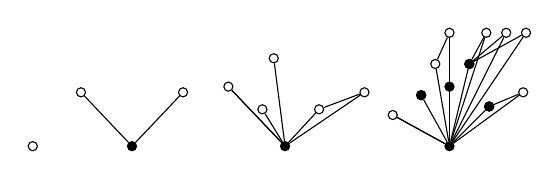
\begin{tikzpicture}[scale=0.72]
  \tikzset{open/.style={circle,draw,fill=white,inner sep=0pt,minimum size=3.3pt}, solid/.style={circle,draw,fill=black,inner sep=0pt,minimum size=3.3pt}}
  % Stage 1
  \node[open] at (-5.0,0) {};

  % Stage 2
  \node[solid] (s2b) at (-3.25,0) {};
  \node[open] (s2l) at (-4.15,0.95) {};
  \node[open] (s2r) at (-2.35,0.95) {};
  \draw (s2b)--(s2l) (s2b)--(s2r);

  % Stage 3
  \node[solid] (s3bot) at (-0.55,0) {};
  \foreach \x/\y/\name in {-1.55/1.05/a,-0.95/0.65/b,-0.75/1.55/c,0.05/0.65/d,0.85/0.95/e} {
    \node[open] (s3\name) at (\x,\y) {};
    \draw (s3bot)--(s3\name);
  }
  \draw (s3a)--(s3bot) (s3d)--(s3e);

  % Stage 4
  \node[solid] (s4bot) at (2.35,0) {};
  \foreach \x/\y/\name in {1.35/0.55/a,1.85/0.9/b,2.1/1.45/c,2.35/2.0/d,2.7/1.45/e,3.0/2.0/f,3.35/2.0/g,3.7/2.0/h,3.05/0.7/i,3.65/0.95/j} {
    \node[open] (s4\name) at (\x,\y) {};
    \draw (s4bot)--(s4\name);
  }
  \node[solid] at (1.85,0.9) {};
  \node[solid] at (2.35,1.05) {};
  \node[solid] at (2.7,1.45) {};
  \node[solid] at (3.05,0.7) {};
  \draw (s4a)--(s4bot) (s4i)--(s4j) (s4c)--(s4d) (s4e)--(s4f) (s4e)--(s4g) (s4e)--(s4h);
\end{tikzpicture}
\caption*{Figure 9: An expanding sequence of finite domains.}
\end{figure}

The order on the limit object is inherited from the product, that is, tuples are ordered coordinatewise. It is again a dcpo because the coordinatewise supremum of commuting tuples is commuting as all $f_j$ are Scott-continuous. This also proves that the projections $\pi_j:\prod_{i\in O}D_i\to D_j$ restricted to $D$ are continuous. They give us the maps needed to complement $D$ to a cone.

Given any other cone $\langle E,(g_i:E\to D_i)_{i\in O}\rangle$, we define the mediating morphism $h:E\to D$ by $h(x)=\langle g_i(x):i\in O\rangle$. Again, it is obvious that this is well-defined and continuous, and that it is the only possible choice.

We also have the dual:

\sourcepage{47}
\leanmarker{thm-3-3-2}{Theorem 3.3.2} $\mathbf{DCPO}$ has colimits of arbitrary diagrams.

This was first noted in [Mar77] and, for a somewhat different setting, in [Mes77]. The simplest way to prove it is by reducing it to completeness \`a la Theorem 23.14 of [HS73]. This appears in [LS81]. A more detailed analysis of colimits appears in [Fie92]. There the problem of retaining algebraicity is also addressed.

\leanmarker{thm-3-3-3}{Theorem 3.3.3} $\mathbf{DCPO}$ is cartesian closed, complete and cocomplete.

\leanmarker{thm-3-3-4}{Theorem 3.3.4} $\mathbf{DCPO}_{\bot!}$ is monoidal closed, complete and cocomplete.

How about $\mathbf{DCPO}_{\bot}$, where objects have least elements but morphisms need not preserve them? The truth is that both completeness and cocompleteness fail for this category. On the other hand, it is the right setting for denotational semantics in most cases. As a result of this mismatch, we quite often must resort to detailed proofs on the element level and cannot simply apply general category theoretic principles. Let us nevertheless write down the one good property of $\mathbf{DCPO}_{\bot}$:

\leanmarker{thm-3-3-5}{Theorem 3.3.5} $\mathbf{DCPO}_{\bot}$ is cartesian closed.

\sourcepage{48}
\leanmarker{def-3-3-6}{Definition 3.3.6} A diagram
\[
  \langle (D_n)_{n\in\mathbb{N}},\ (e_{mn}:D_n\to D_m)_{n\le m\in\mathbb{N}}\rangle
\]
in the category $\mathbf{DCPO}$ is called an \emph{expanding sequence}, if the following conditions are satisfied:
\begin{enumerate}
\item Each $e_{mn}:D_n\to D_m$ is an embedding. The associated projection $e^*_{mn}$ is denoted by $p_{nm}$.
\item $\forall n\in\mathbb{N}.\ e_{nn}=\operatorname{id}_{D_n}$.
\item $\forall n\le m\le k\in\mathbb{N}.\ e_{kn}=e_{km}\circ e_{mn}$.
\end{enumerate}
Note that because lower adjoints determine upper adjoints and vice versa, we have $p_{nk}=p_{nm}\circ p_{mk}$ whenever $n\le m\le k\in\mathbb{N}$.

It turns out that, in contrast to the general situation, the colimit of an expanding sequence can be calculated easily via the associated projections.

\leanmarker{thm-3-3-7}{Theorem 3.3.7} Let
\[
  \langle (D_n)_{n\in\mathbb{N}},\ (e_{mn}:D_n\to D_m)_{n\le m\in\mathbb{N}}\rangle
\]
be an expanding sequence in $\mathbf{DCPO}$. Define an object $D$ by
\[
  D=\{\langle x_n:n\in\mathbb{N}\rangle\in\prod_{n\in\mathbb{N}}D_n
      \mid \forall n\le m\in\mathbb{N}.\ x_n=p_{nm}(x_m)\},
\]
projections $p_m:D\to D_m$ by $\langle x_n:n\in\mathbb{N}\rangle\mapsto x_m$, and embeddings $e_m:D_m\to D$ by
\[
  x\mapsto \left\langle \bigvee^{\uparrow}_{k\ge n,m} p_{nk}\circ e_{km}(x):n\in\mathbb{N}\right\rangle.
\]
Then:
\begin{enumerate}
\item The maps $(e_m,p_m)$, $m\in\mathbb{N}$, form embedding projection pairs and
\[
  \bigvee^{\uparrow}_{m\in\mathbb{N}} e_m\circ p_m=\operatorname{id}_D
\]
holds.
\item $\langle D,(p_n)_{n\in\mathbb{N}}\rangle$ is a limit of the diagram $\langle(D_n)_{n\in\mathbb{N}},(p_{nm})_{n\le m\in\mathbb{N}}\rangle$. If $\langle C,(g_n)_{n\in\mathbb{N}}\rangle$ is another cone, then the mediating map from $C$ to $D$ is given by
\[
  g(x)=\langle g_n(x):n\in\mathbb{N}\rangle
  \quad\text{or}\quad
  g=\bigvee^{\uparrow}_{n\in\mathbb{N}} e_n\circ g_n.
\]
\item $\langle D,(e_n)_{n\in\mathbb{N}}\rangle$ is a colimit of the diagram $\langle(D_n)_{n\in\mathbb{N}},(e_{mn})_{n\le m\in\mathbb{N}}\rangle$. If $\langle E,(f_n)_{n\in\mathbb{N}}\rangle$ is another cocone, then the mediating map from $D$ to $E$ is given by
\[
  f(\langle x_n:n\in\mathbb{N}\rangle)=\bigvee^{\uparrow}_{n\in\mathbb{N}}f_n(x_n)
  \quad\text{or}\quad
  f=\bigvee^{\uparrow}_{n\in\mathbb{N}}f_n\circ p_n.
\]
\end{enumerate}
The directed supremum in the definition of $e_m$ could be replaced by $p_{nk}\circ e_{km}(x)$ for any upper bound $k$ of $\{n,m\}$ in $\mathbb{N}$; the displayed form makes the proof uniform.

\emph{Proof sketch.} The limiting part follows from Theorem 3.3.1 applied to the projection diagram. The tuple defining $e_m(x)$ is commuting by the projection equations, and the assignment is Scott-continuous because it is built from Scott-continuous maps and directed suprema. A direct calculation gives $p_m\circ e_m=\operatorname{id}$ and $e_m\circ p_m\sqsubseteq\operatorname{id}_D$; a closer coordinatewise analysis shows that the directed supremum of the endomaps $e_m\circ p_m$ is the identity. The universal property of the colimit follows by defining the mediating map as $\bigvee^{\uparrow}_{n\in\mathbb{N}}f_n\circ p_n$, using directedness of the family $f_n\circ p_n$, and uniqueness follows by composing with the approximating idempotents $e_m\circ p_m$.

This fact, that the colimit of an expanding sequence is canonically isomorphic to the limit of the associated dual diagram, is called the \emph{limit-colimit coincidence}. It is one of the fundamental tools of domain theory and plays its most prominent role in the solution of recursive domain equations, Chapter 5. Because of this coincidence we will henceforth also speak of the \emph{bilimit} of an expanding sequence and denote it by $\operatorname{bilim}\langle(D_n),(e_{mn})\rangle$.

\sourcepage{50}
\leanmarker{lemma-3-3-8}{Lemma 3.3.8} Let $\langle E,(f_n)_{n\in\mathbb{N}}\rangle$ be a cocone for the expanding sequence
\[
  \langle(D_n)_{n\in\mathbb{N}},(e_{mn}:D_n\to D_m)_{n\le m\in\mathbb{N}}\rangle.
\]
It is colimiting if and only if, firstly, there are Scott-continuous functions $g_n:E\to D_n$ such that each $(f_n,g_n)$ is an e-p-pair and, secondly,
\[
  \bigvee^{\uparrow}_{n\in\mathbb{N}} f_n\circ g_n=\operatorname{id}_E
\]
holds.

\emph{Proof.} Necessity is Part (1) of Theorem 3.3.7. For sufficiency we show that the bilimit $D$ as constructed there is isomorphic to $E$. We already have maps $f:D\to E$ and $g:E\to D$ because $D$ is the bilimit. These commute with the limiting and colimiting morphisms, respectively. Their composites are identities:
\[
  f\circ g(x)=f(\langle g_n(x):n\in\mathbb{N}\rangle)
    =\bigvee^{\uparrow}_{n\in\mathbb{N}}f_n\circ g_n(x)=x,
\]
and
\[
\begin{aligned}
  g\circ f
  &=\left(\bigvee^{\uparrow}_{n\in\mathbb{N}}e_n\circ g_n\right)\circ
    \left(\bigvee^{\uparrow}_{m\in\mathbb{N}}f_m\circ p_m\right)\\
  &=\bigvee^{\uparrow}_{n\in\mathbb{N}} e_n\circ g_n\circ f_n\circ p_n\\
  &=\bigvee^{\uparrow}_{n\in\mathbb{N}} e_n\circ p_n
    =\operatorname{id}_D.
\end{aligned}
\]
We note that in the proof we have used the condition $\bigvee^{\uparrow}_{n\in\mathbb{N}}f_n\circ g_n=\operatorname{id}_E$ only for the first calculation. Without it, we still get that $f$ and $g$ form an e-p-pair. Thus we have:

\sourcepage{51}
\leanmarker{prop-3-3-9}{Proposition 3.3.9} Let $\langle E,(f_n)_{n\in\mathbb{N}}\rangle$ be a cocone over the expanding sequence
\[
  \langle(D_n)_{n\in\mathbb{N}},(e_{mn}:D_n\to D_m)_{n\le m\in\mathbb{N}}\rangle
\]
where the $f_n$ are embeddings. Then the bilimit of the sequence is a sub-domain of $E$.

In other words:

\leanmarker{cor-3-3-10}{Corollary 3.3.10} The bilimit of an expanding sequence is also the colimit (limit) in the restricted category of dcpo's with embeddings (projections) as morphisms.

\leanmarker{thm-3-3-11}{Theorem 3.3.11} Let
\[
  \langle(D_n)_{n\in\mathbb{N}},(e_{mn}:D_n\to D_m)_{n\le m\in\mathbb{N}}\rangle
\]
be an expanding sequence and $\langle D,(e_n)_{n\in\mathbb{N}}\rangle$ its bilimit.
\begin{enumerate}
\item If all $D_n$ are $(\omega\text{-})$continuous then so is $D$. If we are given bases $B_n$, $n\in\mathbb{N}$, for each $D_n$, then a basis for $D$ is given by
\[
  \bigcup_{n\in\mathbb{N}} e_n(B_n).
\]
\item If all $D_n$ are $(\omega\text{-})$algebraic then so is $D$ and
\[
  K(D)=\bigcup_{n\in\mathbb{N}}e_n(K(D_n)).
\]
\end{enumerate}

\emph{Proof.} Given an element $x\in D$ we first show that
\[
  \bigcup_{n\in\mathbb{N}} e_n(B_{p_n(x)}^n)
\]
is directed. It is sufficient to show that for all $n\le m\in\mathbb{N}$ and for each $y\in B_{p_n(x)}^n$ there is $y'\in B_{p_m(x)}^m$ with $e_n(y)\sqsubseteq e_m(y')$. Since $y\ll p_n(x)$ and embeddings preserve approximation,
\[
  e_{mn}(y)\ll e_{mn}(p_n(x))=e_{mn}(p_{nm}\circ p_m(x))\sqsubseteq p_m(x).
\]
As $p_m(x)=\bigvee^{\uparrow}B_{p_m(x)}^m$, some $y'\ll p_m(x)$ is above $e_{mn}(y)$, and hence $e_n(y)=e_m(e_{mn}(y))\sqsubseteq e_m(y')$.

The set $\bigcup_{n\in\mathbb{N}}e_n(B_{p_n(x)}^n)$ gives back $x$ because
\[
  x=\bigvee^{\uparrow}_{n\in\mathbb{N}}e_n\circ p_n(x)
   =\bigvee^{\uparrow}_{n\in\mathbb{N}}e_n\left(\bigvee^{\uparrow}B_{p_n(x)}^n\right)
   =\bigvee^{\uparrow}\bigcup_{n\in\mathbb{N}}e_n(B_{p_n(x)}^n).
\]
It consists solely of approximants to $x$ because the $e_n$ are lower adjoints.

\end{document}
